% Autor: Elias Welt
\section{Lernkarten (Flashcards.jsx)}

Die Flashcard-Komponente ermöglicht klassisches Karteikarten-Lernen mit einem markanten 3D-Flip-Effekt. Sie demonstriert den gezielten Einsatz von CSS-Transformationen und einer unkonventionellen, aber effizienten State-Struktur.

\begin{figure}[h]
    \centering
    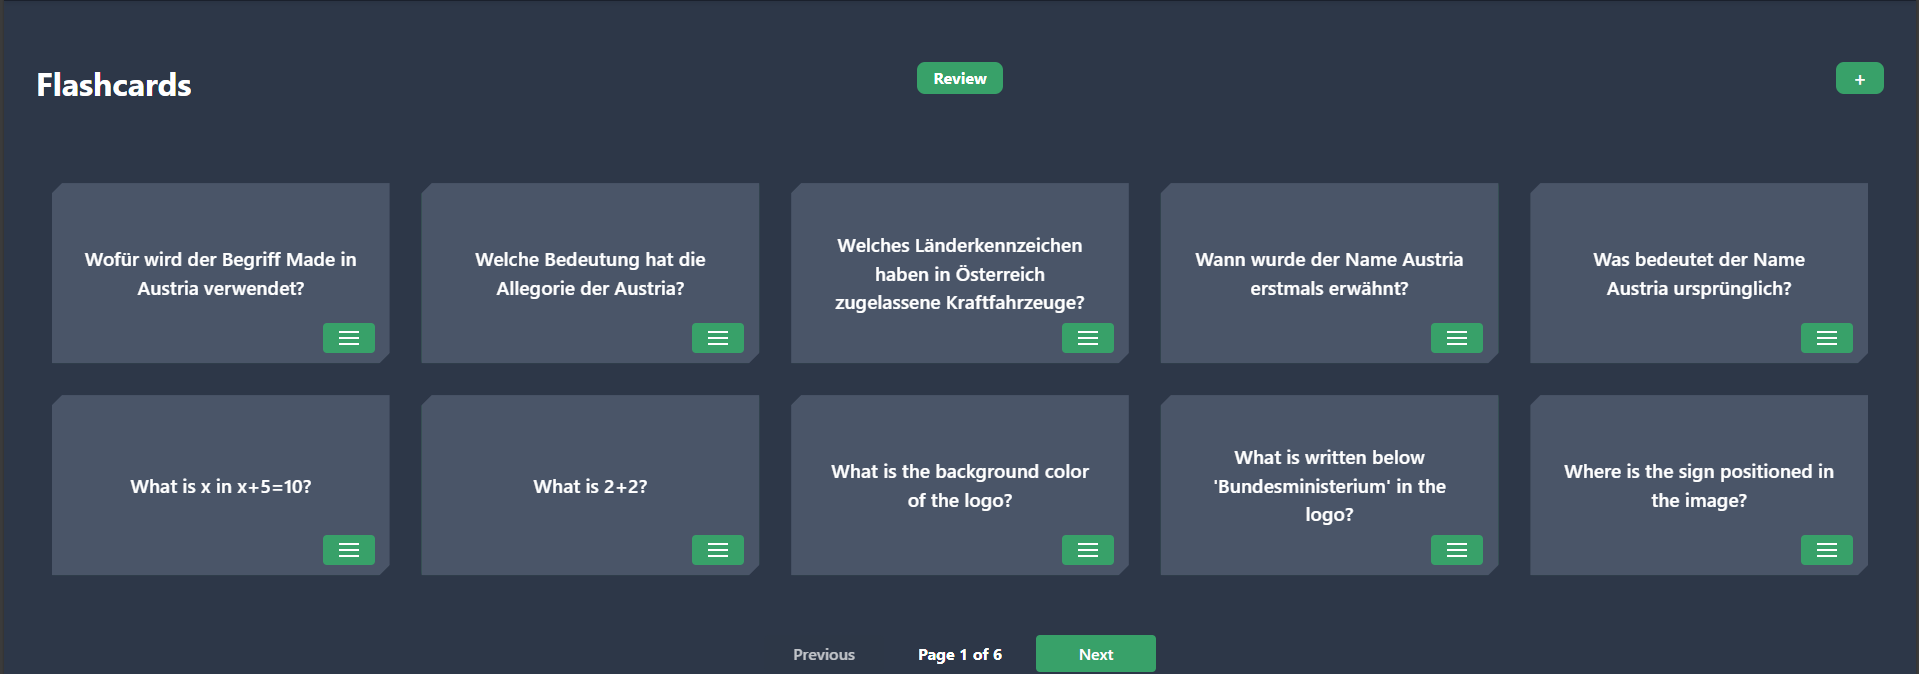
\includegraphics[width=0.92\textwidth]{img/flashcards-dark-mode}
    \caption{Lernkarten-Ansicht von EduShelf im Dark-Mode}
    \label{fig:flashcards}
\end{figure}


\subsection{CSS 3D-Flip-Effekt}

Der realistische Dreh-Effekt wird ausschließlich über CSS 3D-Transformationen realisiert -- ohne JavaScript-Animation. Das Schlüsselelement ist die \texttt{perspective}-Eigenschaft, die dem Browser mitteilt, aus welcher Entfernung der 3D-Raum betrachtet wird:

\begin{lstlisting}[language=CSS, caption={CSS für den 3D-Flip-Effekt}]
.flashcard-scene {
  perspective: 1000px;
}
.flashcard-container {
  transition: transform 0.6s;
  transform-style: preserve-3d;
}
.flashcard-scene.flipped .flashcard-container {
  transform: rotateY(180deg);
}
\end{lstlisting}

Vor- und Rückseite der Karte sind übereinander gestapelt. Die Rückseite ist initial um 180° um die Y-Achse gedreht und somit unsichtbar. Durch Hinzufügen der CSS-Klasse \texttt{.flipped} dreht sich die gesamte Karte, was die Vorderseite verbirgt und die Rückseite sichtbar macht.

\subsection{State-Verwaltung mit einem Set}

Anstatt für jede Karte einen Boolean im Datenobjekt zu speichern, wird ein \texttt{Set} verwendet, das die IDs der umgedrehten Karten hält. Diese Trennung von UI-Zustand und Daten ist ein wichtiges Designprinzip:

\begin{lstlisting}[language=JavaScript, caption={Nutzung eines Sets für UI-Zustand}]
const [flippedCards, setFlippedCards] = useState(new Set());

const flipCard = (id) => {
    setFlippedCards(prevFlippedCards => {
        const newFlippedCards = new Set(prevFlippedCards);
        if (newFlippedCards.has(id)) {
            newFlippedCards.delete(id);
        } else {
            newFlippedCards.add(id);
        }
        return newFlippedCards;
    });
};
\end{lstlisting}

Beim Rendern wird \texttt{flippedCards.has(card.id)} geprüft, um die CSS-Klasse \texttt{.flipped} bedingt hinzuzufügen. Diese Methode erlaubt es, beliebig viele Karten gleichzeitig umgedreht zu halten, ohne das Datenmodell zu verändern.
\newpage

